\documentclass[]{article}
\usepackage{lmodern}
\usepackage{amssymb,amsmath}
\usepackage{ifxetex,ifluatex}
\usepackage{fixltx2e} % provides \textsubscript
\ifnum 0\ifxetex 1\fi\ifluatex 1\fi=0 % if pdftex
  \usepackage[T1]{fontenc}
  \usepackage[utf8]{inputenc}
\else % if luatex or xelatex
  \ifxetex
    \usepackage{mathspec}
  \else
    \usepackage{fontspec}
  \fi
  \defaultfontfeatures{Ligatures=TeX,Scale=MatchLowercase}
\fi
% use upquote if available, for straight quotes in verbatim environments
\IfFileExists{upquote.sty}{\usepackage{upquote}}{}
% use microtype if available
\IfFileExists{microtype.sty}{%
\usepackage{microtype}
\UseMicrotypeSet[protrusion]{basicmath} % disable protrusion for tt fonts
}{}
\usepackage[margin=1in]{geometry}
\usepackage{hyperref}
\hypersetup{unicode=true,
            pdftitle={WGCNA Demo},
            pdfauthor={Shaurya Jauhari (Email: shauryajauhari@gzhmu.edu.cn)},
            pdfborder={0 0 0},
            breaklinks=true}
\urlstyle{same}  % don't use monospace font for urls
\usepackage{color}
\usepackage{fancyvrb}
\newcommand{\VerbBar}{|}
\newcommand{\VERB}{\Verb[commandchars=\\\{\}]}
\DefineVerbatimEnvironment{Highlighting}{Verbatim}{commandchars=\\\{\}}
% Add ',fontsize=\small' for more characters per line
\usepackage{framed}
\definecolor{shadecolor}{RGB}{248,248,248}
\newenvironment{Shaded}{\begin{snugshade}}{\end{snugshade}}
\newcommand{\AlertTok}[1]{\textcolor[rgb]{0.94,0.16,0.16}{#1}}
\newcommand{\AnnotationTok}[1]{\textcolor[rgb]{0.56,0.35,0.01}{\textbf{\textit{#1}}}}
\newcommand{\AttributeTok}[1]{\textcolor[rgb]{0.77,0.63,0.00}{#1}}
\newcommand{\BaseNTok}[1]{\textcolor[rgb]{0.00,0.00,0.81}{#1}}
\newcommand{\BuiltInTok}[1]{#1}
\newcommand{\CharTok}[1]{\textcolor[rgb]{0.31,0.60,0.02}{#1}}
\newcommand{\CommentTok}[1]{\textcolor[rgb]{0.56,0.35,0.01}{\textit{#1}}}
\newcommand{\CommentVarTok}[1]{\textcolor[rgb]{0.56,0.35,0.01}{\textbf{\textit{#1}}}}
\newcommand{\ConstantTok}[1]{\textcolor[rgb]{0.00,0.00,0.00}{#1}}
\newcommand{\ControlFlowTok}[1]{\textcolor[rgb]{0.13,0.29,0.53}{\textbf{#1}}}
\newcommand{\DataTypeTok}[1]{\textcolor[rgb]{0.13,0.29,0.53}{#1}}
\newcommand{\DecValTok}[1]{\textcolor[rgb]{0.00,0.00,0.81}{#1}}
\newcommand{\DocumentationTok}[1]{\textcolor[rgb]{0.56,0.35,0.01}{\textbf{\textit{#1}}}}
\newcommand{\ErrorTok}[1]{\textcolor[rgb]{0.64,0.00,0.00}{\textbf{#1}}}
\newcommand{\ExtensionTok}[1]{#1}
\newcommand{\FloatTok}[1]{\textcolor[rgb]{0.00,0.00,0.81}{#1}}
\newcommand{\FunctionTok}[1]{\textcolor[rgb]{0.00,0.00,0.00}{#1}}
\newcommand{\ImportTok}[1]{#1}
\newcommand{\InformationTok}[1]{\textcolor[rgb]{0.56,0.35,0.01}{\textbf{\textit{#1}}}}
\newcommand{\KeywordTok}[1]{\textcolor[rgb]{0.13,0.29,0.53}{\textbf{#1}}}
\newcommand{\NormalTok}[1]{#1}
\newcommand{\OperatorTok}[1]{\textcolor[rgb]{0.81,0.36,0.00}{\textbf{#1}}}
\newcommand{\OtherTok}[1]{\textcolor[rgb]{0.56,0.35,0.01}{#1}}
\newcommand{\PreprocessorTok}[1]{\textcolor[rgb]{0.56,0.35,0.01}{\textit{#1}}}
\newcommand{\RegionMarkerTok}[1]{#1}
\newcommand{\SpecialCharTok}[1]{\textcolor[rgb]{0.00,0.00,0.00}{#1}}
\newcommand{\SpecialStringTok}[1]{\textcolor[rgb]{0.31,0.60,0.02}{#1}}
\newcommand{\StringTok}[1]{\textcolor[rgb]{0.31,0.60,0.02}{#1}}
\newcommand{\VariableTok}[1]{\textcolor[rgb]{0.00,0.00,0.00}{#1}}
\newcommand{\VerbatimStringTok}[1]{\textcolor[rgb]{0.31,0.60,0.02}{#1}}
\newcommand{\WarningTok}[1]{\textcolor[rgb]{0.56,0.35,0.01}{\textbf{\textit{#1}}}}
\usepackage{graphicx,grffile}
\makeatletter
\def\maxwidth{\ifdim\Gin@nat@width>\linewidth\linewidth\else\Gin@nat@width\fi}
\def\maxheight{\ifdim\Gin@nat@height>\textheight\textheight\else\Gin@nat@height\fi}
\makeatother
% Scale images if necessary, so that they will not overflow the page
% margins by default, and it is still possible to overwrite the defaults
% using explicit options in \includegraphics[width, height, ...]{}
\setkeys{Gin}{width=\maxwidth,height=\maxheight,keepaspectratio}
\IfFileExists{parskip.sty}{%
\usepackage{parskip}
}{% else
\setlength{\parindent}{0pt}
\setlength{\parskip}{6pt plus 2pt minus 1pt}
}
\setlength{\emergencystretch}{3em}  % prevent overfull lines
\providecommand{\tightlist}{%
  \setlength{\itemsep}{0pt}\setlength{\parskip}{0pt}}
\setcounter{secnumdepth}{0}
% Redefines (sub)paragraphs to behave more like sections
\ifx\paragraph\undefined\else
\let\oldparagraph\paragraph
\renewcommand{\paragraph}[1]{\oldparagraph{#1}\mbox{}}
\fi
\ifx\subparagraph\undefined\else
\let\oldsubparagraph\subparagraph
\renewcommand{\subparagraph}[1]{\oldsubparagraph{#1}\mbox{}}
\fi

%%% Use protect on footnotes to avoid problems with footnotes in titles
\let\rmarkdownfootnote\footnote%
\def\footnote{\protect\rmarkdownfootnote}

%%% Change title format to be more compact
\usepackage{titling}

% Create subtitle command for use in maketitle
\providecommand{\subtitle}[1]{
  \posttitle{
    \begin{center}\large#1\end{center}
    }
}

\setlength{\droptitle}{-2em}

  \title{WGCNA Demo}
    \pretitle{\vspace{\droptitle}\centering\huge}
  \posttitle{\par}
    \author{Shaurya Jauhari (Email:
\href{mailto:shauryajauhari@gzhmu.edu.cn}{\nolinkurl{shauryajauhari@gzhmu.edu.cn}})}
    \preauthor{\centering\large\emph}
  \postauthor{\par}
      \predate{\centering\large\emph}
  \postdate{\par}
    \date{2019-10-24}


\begin{document}
\maketitle

Installing the package and setting up the options.

\begin{Shaded}
\begin{Highlighting}[]
\KeywordTok{install.packages}\NormalTok{(}\StringTok{"BiocManager"}\NormalTok{, }
                 \DataTypeTok{repos=}\StringTok{'http://cran.us.r-project.org'}\NormalTok{,}
                 \DataTypeTok{dependencies =} \OtherTok{TRUE}\NormalTok{)}
\end{Highlighting}
\end{Shaded}

\begin{verbatim}
## Installing package into 'C:/Users/rajni/Documents/R/win-library/3.6'
## (as 'lib' is unspecified)
\end{verbatim}

\begin{verbatim}
## Warning: dependency 'BiocStyle' is not available
\end{verbatim}

\begin{verbatim}
## 
##   There is a binary version available but the source version is
##   later:
##             binary source needs_compilation
## BiocManager 1.30.8 1.30.9             FALSE
\end{verbatim}

\begin{verbatim}
## installing the source package 'BiocManager'
\end{verbatim}

\begin{Shaded}
\begin{Highlighting}[]
\NormalTok{BiocManager}\OperatorTok{::}\KeywordTok{install}\NormalTok{(}\StringTok{"WGCNA"}\NormalTok{)}
\end{Highlighting}
\end{Shaded}

\begin{verbatim}
## Bioconductor version 3.9 (BiocManager 1.30.9), R 3.6.0 (2019-04-26)
\end{verbatim}

\begin{verbatim}
## Installing package(s) 'WGCNA'
\end{verbatim}

\begin{verbatim}
## package 'WGCNA' successfully unpacked and MD5 sums checked
## 
## The downloaded binary packages are in
##  C:\Users\rajni\AppData\Local\Temp\RtmpYvzLdm\downloaded_packages
\end{verbatim}

\begin{verbatim}
## Installation path not writeable, unable to update packages: boot, cluster,
##   foreign, KernSmooth, mgcv, nlme
\end{verbatim}

\begin{verbatim}
## Old packages: 'covr', 'data.table', 'DescTools', 'digest', 'lava',
##   'limma', 'markdown', 'modelr', 'pkgbuild', 'pkgconfig', 'promises',
##   'purrr', 'Rcpp', 'recipes', 'reticulate', 'rmarkdown', 'RSQLite',
##   'S4Vectors', 'shiny', 'sys', 'tensorflow', 'testthat', 'tidyr',
##   'tinytex', 'whisker', 'xfun', 'xml2'
\end{verbatim}

\begin{Shaded}
\begin{Highlighting}[]
\KeywordTok{install.packages}\NormalTok{(}\StringTok{"ggdendro"}\NormalTok{, }
                 \DataTypeTok{repos=}\StringTok{'http://cran.us.r-project.org'}\NormalTok{,}
                 \DataTypeTok{dependencies =} \OtherTok{TRUE}\NormalTok{)}
\end{Highlighting}
\end{Shaded}

\begin{verbatim}
## Installing package into 'C:/Users/rajni/Documents/R/win-library/3.6'
## (as 'lib' is unspecified)
\end{verbatim}

\begin{verbatim}
## package 'ggdendro' successfully unpacked and MD5 sums checked
## 
## The downloaded binary packages are in
##  C:\Users\rajni\AppData\Local\Temp\RtmpYvzLdm\downloaded_packages
\end{verbatim}

\begin{Shaded}
\begin{Highlighting}[]
\CommentTok{## Setting options}

\KeywordTok{options}\NormalTok{(}\DataTypeTok{stringsAsFactors =} \OtherTok{FALSE}\NormalTok{)}

\CommentTok{#enableWGCNAThreads() ## Enabling multi-threads in processing.}

\KeywordTok{library}\NormalTok{(WGCNA)}
\end{Highlighting}
\end{Shaded}

\begin{verbatim}
## Warning: package 'WGCNA' was built under R version 3.6.1
\end{verbatim}

\begin{verbatim}
## Loading required package: dynamicTreeCut
\end{verbatim}

\begin{verbatim}
## Loading required package: fastcluster
\end{verbatim}

\begin{verbatim}
## 
## Attaching package: 'fastcluster'
\end{verbatim}

\begin{verbatim}
## The following object is masked from 'package:stats':
## 
##     hclust
\end{verbatim}

\begin{verbatim}
## 
\end{verbatim}

\begin{verbatim}
## 
## Attaching package: 'WGCNA'
\end{verbatim}

\begin{verbatim}
## The following object is masked from 'package:stats':
## 
##     cor
\end{verbatim}

\begin{Shaded}
\begin{Highlighting}[]
\KeywordTok{library}\NormalTok{(ggdendro)}
\end{Highlighting}
\end{Shaded}

\begin{verbatim}
## Warning: package 'ggdendro' was built under R version 3.6.1
\end{verbatim}

\begin{Shaded}
\begin{Highlighting}[]
\KeywordTok{library}\NormalTok{(ggplot2)}
\end{Highlighting}
\end{Shaded}

\begin{verbatim}
## Warning: package 'ggplot2' was built under R version 3.6.1
\end{verbatim}

Importing data files from female and male liver tissues from mice, and
exploring them.

\begin{Shaded}
\begin{Highlighting}[]
\NormalTok{mydataf <-}\StringTok{ }\KeywordTok{read.csv}\NormalTok{(}\StringTok{"./FemaleLiver-Data/LiverFemale3600.csv"}\NormalTok{, }\DataTypeTok{header =} \OtherTok{TRUE}\NormalTok{) }
\KeywordTok{colnames}\NormalTok{(mydataf)}
\end{Highlighting}
\end{Shaded}

\begin{verbatim}
##   [1] "substanceBXH"   "gene_symbol"    "LocusLinkID"    "ProteomeID"    
##   [5] "cytogeneticLoc" "CHROMOSOME"     "StartPosition"  "EndPosition"   
##   [9] "F2_2"           "F2_3"           "F2_14"          "F2_15"         
##  [13] "F2_19"          "F2_20"          "F2_23"          "F2_24"         
##  [17] "F2_26"          "F2_37"          "F2_42"          "F2_43"         
##  [21] "F2_45"          "F2_46"          "F2_47"          "F2_48"         
##  [25] "F2_51"          "F2_52"          "F2_54"          "F2_63"         
##  [29] "F2_65"          "F2_66"          "F2_68"          "F2_69"         
##  [33] "F2_70"          "F2_71"          "F2_72"          "F2_78"         
##  [37] "F2_79"          "F2_80"          "F2_81"          "F2_83"         
##  [41] "F2_86"          "F2_87"          "F2_88"          "F2_89"         
##  [45] "F2_107"         "F2_108"         "F2_109"         "F2_110"        
##  [49] "F2_111"         "F2_112"         "F2_117"         "F2_119"        
##  [53] "F2_125"         "F2_126"         "F2_127"         "F2_141"        
##  [57] "F2_142"         "F2_143"         "F2_144"         "F2_145"        
##  [61] "F2_154"         "F2_155"         "F2_156"         "F2_157"        
##  [65] "F2_162"         "F2_163"         "F2_164"         "F2_165"        
##  [69] "F2_166"         "F2_167"         "F2_169"         "F2_180"        
##  [73] "F2_181"         "F2_182"         "F2_187"         "F2_188"        
##  [77] "F2_189"         "F2_190"         "F2_191"         "F2_192"        
##  [81] "F2_194"         "F2_195"         "F2_200"         "F2_201"        
##  [85] "F2_212"         "F2_213"         "F2_214"         "F2_215"        
##  [89] "F2_221"         "F2_222"         "F2_223"         "F2_224"        
##  [93] "F2_225"         "F2_226"         "F2_227"         "F2_228"        
##  [97] "F2_241"         "F2_242"         "F2_243"         "F2_244"        
## [101] "F2_245"         "F2_247"         "F2_248"         "F2_261"        
## [105] "F2_263"         "F2_264"         "F2_270"         "F2_271"        
## [109] "F2_272"         "F2_278"         "F2_287"         "F2_288"        
## [113] "F2_289"         "F2_290"         "F2_291"         "F2_296"        
## [117] "F2_298"         "F2_299"         "F2_300"         "F2_302"        
## [121] "F2_303"         "F2_304"         "F2_305"         "F2_306"        
## [125] "F2_307"         "F2_308"         "F2_309"         "F2_310"        
## [129] "F2_311"         "F2_312"         "F2_320"         "F2_321"        
## [133] "F2_323"         "F2_324"         "F2_325"         "F2_326"        
## [137] "F2_327"         "F2_328"         "F2_329"         "F2_330"        
## [141] "F2_332"         "F2_355"         "F2_357"
\end{verbatim}

\begin{Shaded}
\begin{Highlighting}[]
\KeywordTok{head}\NormalTok{(mydataf)}
\end{Highlighting}
\end{Shaded}

\begin{verbatim}
##   substanceBXH   gene_symbol LocusLinkID ProteomeID cytogeneticLoc
## 1  MMT00000044 1700007N18Rik       69339     286025              0
## 2  MMT00000046         Mast2       17776     157466              0
## 3  MMT00000051       Ankrd32      105377     321939              0
## 4  MMT00000076             0      383154          0              0
## 5  MMT00000080          Ldb2       16826     157383              0
## 6  MMT00000102          Rdhs      216453          0     10_70.0_cM
##   CHROMOSOME StartPosition EndPosition     F2_2    F2_3     F2_14    F2_15
## 1         16      50911260    50912491 -0.01810  0.0642  6.44e-05 -0.05800
## 2          4     115215318   115372404 -0.07730 -0.0297  1.12e-01 -0.05890
## 3         13      74940309    74982847 -0.02260  0.0617 -1.29e-01  0.08710
## 4         16      49345114    49477048 -0.00924 -0.1450  2.87e-02 -0.04390
## 5          5      43546124    43613704 -0.04870  0.0582 -4.83e-02 -0.03710
## 6         10       1337265     1347607  0.17600 -0.1890 -6.50e-02 -0.00846
##      F2_19       F2_20    F2_23    F2_24   F2_26    F2_37        F2_42
## 1  0.04830 -0.15197410 -0.00129 -0.23600 -0.0307 -0.02610  0.073705890
## 2  0.04430 -0.09380000  0.09340  0.02690 -0.1330  0.07570 -0.009193803
## 3 -0.11500 -0.06502607  0.00249 -0.10200  0.1420 -0.10200  0.064289290
## 4  0.00425 -0.23610000 -0.06900  0.01440  0.0363 -0.01820  0.477874600
## 5  0.02510  0.08504274  0.04450  0.00167 -0.0680  0.00567 -0.075348680
## 6 -0.00574 -0.01807182 -0.12500 -0.06820  0.1250  0.00998 -0.037366600
##     F2_43    F2_45   F2_46    F2_47   F2_48   F2_51   F2_52   F2_54
## 1 -0.0466 -0.00673 -0.0193  0.09040  0.0290  0.0356 -0.0388 -0.0360
## 2 -0.0075  0.01700  0.0722 -0.08390  0.0273 -0.0784 -0.0178  0.1120
## 3  0.0169 -0.01590 -0.1430 -0.00492 -0.0735  0.0657 -0.0197 -0.1290
## 4  0.1440  0.11100  0.0113  0.11900  0.0225  0.0932  0.1430  0.2640
## 5 -0.0673 -0.04720  0.0701 -0.08790 -0.0180 -0.1290 -0.0469 -0.0352
## 6 -0.0402 -0.02190  0.0269  0.13300  0.0732  0.1070 -0.0362 -0.0696
##      F2_63     F2_65   F2_66    F2_68    F2_69    F2_70    F2_71   F2_72
## 1 -0.05600  0.009840 -0.0261  0.00856 -0.01180 -0.03350 -0.08310 -0.0471
## 2  0.12300  0.051700  0.0731  0.08670  0.05710  0.00693 -0.00606 -0.0390
## 3 -0.14300 -0.061600  0.0419 -0.29000 -0.10800 -0.09950 -0.00315  0.0975
## 4 -0.09280 -0.000635 -0.0126  0.06910  0.02260 -0.08630 -0.22900  0.0178
## 5 -0.00166  0.058700 -0.0206 -0.13000  0.00392  0.05450 -0.11200  0.1070
## 6 -0.19400 -0.117000 -0.0400  0.06890  0.04320 -0.00338 -0.05270 -0.0416
##      F2_78        F2_79   F2_80   F2_81   F2_83   F2_86    F2_87    F2_88
## 1 -0.02820  0.047264410  0.0296  0.0114  0.0498 -0.0249 -0.00264 -0.02050
## 2  0.01870  0.008471275 -0.0687 -0.0114 -0.0262 -0.0215 -0.09580 -0.01930
## 3  0.01030 -0.134271000  0.1010  0.0521 -0.0607 -0.0285  0.02560 -0.01350
## 4  0.00166  0.064096960  0.0103 -0.0258 -0.0837  0.1880  0.03310 -0.00652
## 5  0.01190  0.008985630 -0.1030 -0.1400 -0.0282 -0.1090  0.02070 -0.01370
## 6 -0.03040  0.025920240  0.0697  0.1150  0.0953  0.0127  0.05490  0.00311
##     F2_89  F2_107  F2_108   F2_109  F2_110  F2_111  F2_112   F2_117
## 1  0.0826 -0.0421  0.0663  0.03620  0.0808 -0.0404  0.0877  0.07240
## 2 -0.1140  0.0815  0.0285  0.00299 -0.0407 -0.0657  0.0643 -0.00022
## 3  0.0796  0.0553 -0.0380  0.12900 -0.0361  0.0441 -0.1640 -0.01420
## 4  0.1550  0.0458  0.0752  0.12200 -0.0104  0.0914 -0.0355  0.06520
## 5 -0.0288 -0.1220  0.1270 -0.09390  0.1200 -0.0850  0.1400  0.00867
## 6  0.0955 -0.1520 -0.0670 -0.00599 -0.0438  0.0634  0.1380 -0.04010
##    F2_119   F2_125   F2_126   F2_127   F2_141  F2_142   F2_143   F2_144
## 1 -0.0210  0.04540 -0.03220 -0.00654  0.03490 -0.0315 -0.02170  0.00370
## 2 -0.0877  0.00167  0.00321 -0.01260 -0.04530 -0.0579  0.05920  0.00239
## 3 -0.0279  0.00677  0.07360  0.01750  0.10900 -0.0216 -0.01250  0.05460
## 4  0.1280  0.05940  0.01630  0.00292  0.00714 -0.0565  0.10200  0.03480
## 5  0.1440  0.08710 -0.03360  0.17300  0.08270  0.0594 -0.00317 -0.06750
## 6  0.1310 -0.12600  0.00484 -0.00256 -0.06800  0.0941 -0.04220  0.12000
##    F2_145      F2_154    F2_155  F2_156   F2_157   F2_162  F2_163  F2_164
## 1  0.0322 -0.02150730 -0.000958 -0.0850  0.00462  0.03990  0.0716 -0.0923
## 2 -0.0383  0.02457782 -0.030300 -0.1260 -0.06670 -0.00637 -0.0161 -0.2340
## 3  0.0403 -0.01674888  0.059900  0.0311 -0.05190  0.01890  0.0207  0.0929
## 4  0.0245  0.06776892  0.016500 -0.0382  0.02120  0.06690  0.0512 -0.2450
## 5  0.0495  0.13520570  0.016500  0.0832  0.04350  0.19300  0.0586 -0.0768
## 6  0.1080 -0.05128296 -0.005590  0.0136  0.09910  0.06770 -0.0520  0.1550
##     F2_165  F2_166  F2_167   F2_169   F2_180      F2_181  F2_182   F2_187
## 1  0.10900  0.0102  0.0337  0.00911  0.03210  0.03144772  0.0543  0.01120
## 2 -0.09610 -0.1290 -0.0109 -0.11300 -0.00677 -0.16704700 -0.0239  0.00304
## 3  0.00917  0.0874 -0.1260 -0.00949 -0.09900  0.02700180 -0.0570 -0.05160
## 4  1.23000 -0.0402 -0.0635  0.06880  0.03790 -0.02058180  0.0227  0.04180
## 5  0.04600  0.0484  0.2810  0.07210 -0.00630  0.37074790  0.0618  0.10800
## 6  0.07890  0.0336  0.0648  0.14400  0.02770  0.09297908  0.0601  0.02960
##     F2_188  F2_189   F2_190  F2_191  F2_192  F2_194   F2_195  F2_200
## 1  0.01060  0.1130 -0.03960 -0.0504  0.0877 -0.0563 -0.00557 -0.0484
## 2 -0.03580 -0.1330 -0.01830 -0.0623 -0.0648 -0.0652  0.05020 -0.0912
## 3 -0.04970  0.1660  0.05000  0.0498  0.0431 -0.0224 -0.10700  0.0715
## 4  0.01010  0.2170  0.00206 -0.0155  0.6550  0.2820 -0.01310 -0.0387
## 5  0.12100  0.0237  0.02960  0.1130  0.0839  0.1050  0.15500  0.0823
## 6  0.00198  0.0251  0.00059 -0.0282  0.0429  0.0697  0.04930  0.0414
##    F2_201      F2_212  F2_213  F2_214   F2_215  F2_221   F2_222  F2_223
## 1 -0.0273 -0.10816380 -0.0183 -0.0132 -0.00432 -0.6630  0.01440  0.0310
## 2 -0.0180  0.05682362 -0.0238  0.0721  0.03910  0.1070  0.00923 -0.0397
## 3  0.0432 -0.13217820  0.0205 -0.0411  0.07670 -0.0783 -0.06860 -0.0254
## 4 -0.0667 -0.32395020 -0.0245  0.0865  0.06470 -2.0000  0.00874  0.0847
## 5  0.1140  0.03542023 -0.2020  0.0822  0.04260  0.1030 -0.10100  0.1630
## 6 -0.0708 -0.10881230  0.0359 -0.0678 -0.11000 -0.1420  0.08430 -0.0610
##     F2_224   F2_225   F2_226  F2_227  F2_228  F2_241  F2_242   F2_243
## 1  0.00818 -0.00892 -0.08710  0.0129  0.0937  0.0313  0.0821  0.00621
## 2 -0.06400  0.06300 -0.00152  0.0555  0.0947 -0.0387  0.0592 -0.00636
## 3 -0.05680 -0.13300 -0.07560 -0.0557 -0.0890 -0.1460 -0.0739 -0.01120
## 4 -0.09720  0.00746 -0.55200  0.0415  0.0733  0.0815  0.1100  0.21400
## 5  0.07410 -0.01640  0.08700 -0.0557 -0.1910  0.0219  0.0913  0.01120
## 6  0.08760 -0.03960  0.10200  0.0190 -0.1190  0.0687 -0.0525 -0.00716
##    F2_244   F2_245    F2_247       F2_248   F2_261  F2_263   F2_264
## 1  0.0307 -0.13700  0.075300 -0.096881950 -0.01670 -0.0928 -0.00957
## 2  0.0614  0.02850 -0.000633  0.001598228 -0.00267 -0.0198  0.16300
## 3 -0.0528  0.05050  0.027700 -0.067933370 -0.02220 -0.0684 -0.04930
## 4  0.0135 -0.13500 -0.003100  0.072318780  0.01030 -0.3150  0.08420
## 5  0.1190  0.00383  0.041700 -0.038618510  0.11800  0.0123  0.03700
## 6 -0.1460 -0.14500  0.029400  0.035281240 -0.05660  0.0917 -0.08080
##    F2_270   F2_271  F2_272   F2_278  F2_287      F2_288    F2_289  F2_290
## 1  0.0287 -0.01300 -0.0292 -0.03810 -0.0488  0.17361240 -0.097900  0.0383
## 2 -0.1310 -0.04260 -0.0514  0.07260 -0.0481 -0.16211430 -0.123000 -0.1370
## 3  0.0328  0.00537 -0.0259 -0.14400  0.0170  0.25924220 -0.041400 -0.0229
## 4  0.0351       NA  0.0730  0.00914  0.0556  0.18311140  0.051700  0.1780
## 5 -0.0142  0.00563 -0.0504 -0.05970 -0.0871  0.20897910 -0.000188 -0.0328
## 6  0.0362  0.00790 -0.0246 -0.07330  0.0125 -0.04778892  0.082500  0.1360
##     F2_291      F2_296  F2_298   F2_299    F2_300  F2_302  F2_303  F2_304
## 1  0.01850 -0.08937784  0.0230 -0.06250 -0.000142  0.0344  0.0358 -0.0139
## 2 -0.05720 -0.07416870 -0.0688 -0.06540 -0.102000 -0.0780 -0.0820 -0.1830
## 3 -0.00664 -0.05915232 -0.0134  0.09740  0.015500 -0.0934  0.1780  0.0842
## 4  0.05250 -0.21653720 -0.2210 -0.00266  0.545000  0.0127  0.0273 -0.0928
## 5 -0.16600 -0.07897525  0.1410 -0.12900  0.090600 -0.1330 -0.2120 -0.0797
## 6  0.04620  0.03811979 -0.0346  0.04690 -0.034800  0.0110  0.0323  0.1660
##    F2_305      F2_306   F2_307   F2_308  F2_309   F2_310  F2_311  F2_312
## 1  0.0134 -0.03145069  0.02780 -0.01190 -0.0744  0.00197 -0.0151 -0.0721
## 2 -0.0270 -0.09822316 -0.07890 -0.05480 -0.1320 -0.11000 -0.1130 -0.0805
## 3  0.0870  0.15520470  0.03410 -0.06830  0.0555 -0.04060  0.0835  0.0514
## 4  0.0469  0.10038160 -2.00000  0.05240  0.1260  0.07280  0.0600 -0.0455
## 5 -0.0191 -0.11958500  0.00294 -0.10600 -0.0518 -0.13200  0.0494  0.0221
## 6 -0.0866  0.05385017  0.09570 -0.00949  0.1120  0.20800  0.0872 -0.0555
##    F2_320  F2_321  F2_323    F2_324  F2_325  F2_326  F2_327   F2_328
## 1 -0.0118  0.0200  0.0222  0.047700 -0.0488  0.0168 -0.0309  0.02740
## 2 -0.1200  0.0101 -0.1610 -0.049200 -0.0350 -0.0738 -0.1730 -0.07380
## 3  0.0713 -0.1130  0.0466  0.000612  0.1210  0.0996  0.1090  0.02730
## 4 -0.0464  0.0667 -0.1850 -0.270000  0.0803  0.0424  0.1610  0.05120
## 5  0.0272 -0.0938  0.1020  0.113000 -0.0859 -0.1340  0.0639  0.00731
## 6  0.0748 -0.1420  0.0590 -0.080000 -0.1200  0.1230  0.1870  0.05410
##    F2_329  F2_330  F2_332  F2_355    F2_357
## 1 -0.0310  0.0660 -0.0199 -0.0146  0.065000
## 2 -0.2010 -0.0820 -0.0939  0.0192 -0.049900
## 3  0.1200 -0.0629 -0.0395  0.1090  0.000253
## 4  0.2410  0.3890  0.0251 -0.0348  0.114000
## 5  0.1240 -0.0212  0.0870  0.0512  0.024300
## 6  0.0699  0.0708  0.1450 -0.0399  0.037500
\end{verbatim}

\begin{Shaded}
\begin{Highlighting}[]
\NormalTok{mydatam <-}\StringTok{ }\KeywordTok{read.csv}\NormalTok{(}\StringTok{"./LiverMale3600.csv"}\NormalTok{)}
\KeywordTok{head}\NormalTok{(mydatam)}
\end{Highlighting}
\end{Shaded}

\begin{verbatim}
##   substanceBXH   gene_symbol LocusLinkID ProteomeID cytogeneticLoc
## 1  MMT00000044 1700007N18Rik       69339     286025              0
## 2  MMT00000046         Mast2       17776     157466              0
## 3  MMT00000051       Ankrd32      105377     321939              0
## 4  MMT00000076             0      383154          0              0
## 5  MMT00000080          Ldb2       16826     157383              0
## 6  MMT00000102          Rdhs      216453          0     10_70.0_cM
##   CHROMOSOME StartPosition EndPosition    F2_4    F2_5    F2_6     F2_7
## 1         16      50911260    50912491 -0.0444 -0.0179 -0.0431  0.03580
## 2          4     115215318   115372404  0.1250  0.0507  0.1290  0.13900
## 3         13      74940309    74982847 -0.1510 -0.0689 -0.0925  0.00353
## 4         16      49345114    49477048 -0.1650 -0.0285  2.0000  0.04570
## 5          5      43546124    43613704 -0.0724 -0.0603 -0.0569  0.02610
## 6         10       1337265     1347607 -0.1430 -0.0663 -0.1570 -0.23700
##      F2_8     F2_9     F2_10   F2_13   F2_16   F2_17   F2_18   F2_22
## 1  0.0263  0.15400  0.000109  0.0254 -0.0294  0.1160  0.0431 -0.0267
## 2  0.2370 -0.00483  0.007490  0.0227  0.0355  0.0836  0.1230  0.1180
## 3 -0.1610 -0.00932 -0.191000  0.0809  0.0692 -0.1350 -0.0471 -0.0785
## 4 -0.4550  0.33200  0.043500  0.0944  0.1640  0.0774  0.0169 -0.1030
## 5 -0.1130 -0.01210 -0.161000  0.0100 -0.1320 -0.1550 -0.1420 -0.0666
## 6 -0.2090 -0.09170  0.060800 -0.1330 -0.0683 -0.2010 -0.2530 -0.2020
##     F2_27    F2_28   F2_29    F2_30   F2_33   F2_34   F2_35   F2_39
## 1 -0.2160 -0.12700  0.0377 -0.07320 -0.0137  0.0434 -0.0277  0.0667
## 2  0.1200  0.16300  0.1570  0.20600 -0.0102  0.1460  0.1890  0.1170
## 3 -0.0352  0.00584 -0.1070 -0.07020 -0.0273  0.0426  0.0314  0.0751
## 4 -0.2080 -0.25600  0.0204 -0.04560 -0.8740 -0.8230  0.2260  0.1750
## 5 -0.0351 -0.03760 -0.0966  0.00728 -0.0629  0.1210 -0.2050  0.0322
## 6 -0.1110 -0.12700 -0.0948 -0.19000 -0.1610 -0.1260 -0.1760 -0.1850
##     F2_40   F2_41   F2_49       F2_50    F2_55   F2_56   F2_57       F2_59
## 1  0.0283  0.0541  0.0533 -0.06555326 -0.00713  0.0453  0.0256  0.02944015
## 2  0.2400  0.1560  0.0114 -0.02107601  0.10900  0.1700  0.2540  0.08054645
## 3 -0.1070 -0.0586 -0.0698 -0.07634149 -0.03310 -0.0901 -0.0965 -0.11589100
## 4  0.0204  0.0801 -0.0481 -0.17293770  0.13600  0.0427  0.0187  0.35591750
## 5 -0.0158 -0.0989 -0.0752 -0.03223757 -0.06150  0.0164 -0.1050 -0.05905863
## 6 -0.2190 -0.2260  0.0867 -0.08595835 -0.06300 -0.1770 -0.1320 -0.05455500
##     F2_60   F2_73   F2_74   F2_75   F2_76   F2_84   F2_85   F2_91   F2_92
## 1 -0.0459  0.0338 -0.0458  0.0201  0.0300 -0.0352 -0.1050  0.0259  0.0939
## 2  0.1890  0.1640  0.0728  0.1230  0.1360  0.2380  0.1000  0.2040  0.1950
## 3 -0.0930 -0.0391  0.0406 -0.0223 -0.0397 -0.0299 -0.0903 -0.2060 -0.1140
## 4  0.0437 -0.2150 -0.0366  0.0152  0.0448  0.4910 -0.5400  0.0573 -0.0314
## 5 -0.1030  0.0122 -0.1220 -0.0603 -0.0907 -0.0313 -0.0243 -0.2260  0.0257
## 6 -0.2250 -0.1760 -0.0801 -0.1050 -0.1510 -0.1560 -0.1650 -0.0885 -0.2140
##      F2_93       F2_94  F2_104  F2_105   F2_114  F2_115  F2_116   F2_120
## 1  0.04060  0.05805066 -0.0118  0.0143 -0.08070 -0.0418 -0.0559  0.00961
## 2  0.06750 -0.09036969  0.2950 -0.0661 -0.02010  0.0179  0.0837  0.04040
## 3 -0.01200 -0.04731417 -0.1050  0.0588  0.00895  0.1190  0.0474 -0.08880
## 4  0.08910  0.03246458  0.0498  0.0764 -0.07570  0.0532 -0.1520  0.14000
## 5  0.00118 -0.01082061  0.0462  0.0566  0.00530  0.0935 -0.0622  0.05640
## 6 -0.08690 -0.01983479 -0.2880 -0.0425 -0.10000 -0.1520 -0.1490 -0.03080
##     F2_121    F2_122   F2_123   F2_124    F2_146   F2_147  F2_148  F2_149
## 1  0.02130 -0.000128  0.04350  0.01260  0.003750  0.00994 -0.0225  0.0593
## 2  0.15900  0.004370  0.02910  0.05050  0.049400  0.17200 -0.0412  0.0968
## 3 -0.13600  0.052000 -0.00612  0.04040  0.008640  0.02550 -0.0475  0.0802
## 4 -0.03820 -0.041300  0.09380 -0.11600 -0.048700  0.07400  0.0380  0.0568
## 5  0.00566 -0.000152  0.07480 -0.00657 -0.000285  0.13500  0.1200 -0.0286
## 6 -0.10200 -0.093200 -0.04530 -0.16100 -0.085200 -0.18200 -0.0417 -0.1450
##     F2_151  F2_152  F2_153    F2_158  F2_159  F2_160  F2_170   F2_171
## 1 -0.00857  0.0288  0.0761  0.000479 -0.0189  0.0438  0.0149  0.02290
## 2  0.04930 -0.0367 -0.1340  0.138000 -0.0126  0.0757  0.0853  0.14800
## 3  0.04530  0.0184  0.0162 -0.052900  0.0576 -0.0076 -0.0349 -0.03930
## 4 -0.00238 -0.0396  0.0121  0.026400  0.0114  0.0108  0.0861  0.01890
## 5  0.15700 -0.0247  0.1090  0.004630 -0.1240 -0.0387  0.0269  0.00419
## 6 -0.04530 -0.0119  0.0662 -0.063400  0.0423 -0.0895 -0.1090 -0.11600
##    F2_172  F2_173  F2_174   F2_176   F2_178  F2_179   F2_183   F2_184
## 1  0.0812 -0.0100  0.0492  0.03220  0.07230 -0.0196 -0.05150  0.00377
## 2 -0.0538  0.1300  0.1850  0.02230  0.00528  0.0265  0.03850  0.19300
## 3  0.0696  0.0564 -0.0620  0.02440  0.00459 -0.0327  0.00872 -0.04460
## 4  0.0772  0.0169  0.0694  0.00808  0.15500 -0.1810 -0.03080 -0.01700
## 5 -0.0258 -0.1100  0.0790  0.08090 -0.02610 -0.0216 -0.08210  0.03000
## 6  0.0621 -0.1820 -0.1480 -0.09400  0.00701 -0.0180  0.06090 -0.18000
##     F2_185      F2_186   F2_197   F2_198  F2_199  F2_207  F2_208   F2_209
## 1  0.03590  0.02331811  0.08710  0.00320 -0.0152  0.0919  0.0745 -0.07960
## 2  0.06140  0.05443614 -0.09730  0.02270  0.0731  0.1870  0.1540  0.14400
## 3 -0.07370 -0.16528400  0.00276  0.00964 -0.0403 -0.0760 -0.0429 -0.12000
## 4 -0.12100 -0.04767130 -0.06740  0.00838  0.0253  0.2100 -0.3510  0.09110
## 5  0.00615  0.05199314  0.04700  0.04130 -0.0335  0.1610  0.1570  0.00777
## 6  0.00157 -0.05937405 -0.04100 -0.04790 -0.1440 -0.2910 -0.2530 -0.11300
##    F2_210    F2_216  F2_217  F2_218   F2_219  F2_220      F2_230  F2_231
## 1  0.0848 -0.093800 -0.0898  0.0472  0.00513  0.0578  0.05616089  0.1470
## 2  0.0594  0.109000  0.0791  0.2110  0.08110  0.1580  0.19241050  0.1410
## 3 -0.0627 -0.029200  0.1090 -0.0459 -0.06390 -0.1700 -0.09710876 -0.0163
## 4  0.0349 -0.024900 -0.0165  0.7450  0.04310  0.0427  0.38320980  0.1750
## 5  0.0935  0.000275 -0.0371  0.0980  0.07460  0.2250 -0.11742250 -0.0112
## 6 -0.0358 -0.042800 -0.1930 -0.1750 -0.02980 -0.1190 -0.15757000 -0.0319
##      F2_232  F2_233  F2_234      F2_235  F2_236   F2_237   F2_238   F2_239
## 1  0.018600  0.0976  0.0160  0.05150205  0.0394  0.00542 0.000242 -0.01540
## 2  0.056600  0.2570  0.2590  0.14049010  0.0965  0.04190 0.009570  0.11900
## 3 -0.000807 -0.1110 -0.1750 -0.09649123  0.0154 -0.00482 0.014500 -0.00822
## 4 -0.040400  0.0284 -0.1630  0.02090355  0.0610  0.04090 0.004970  0.19500
## 5  0.007410  0.2130  0.0578  0.06377663 -0.0739 -0.03110 0.019900 -0.02510
## 6 -0.046300 -0.2130 -0.2990 -0.10599170 -0.0209 -0.14300 0.069700 -0.08810
##     F2_249  F2_250  F2_251    F2_252   F2_254      F2_256      F2_257
## 1 -0.02430 -0.1010  0.0626 -0.060100  0.11600  0.03889860  0.07270702
## 2  0.08050  0.1460  0.0296  0.243000  0.18900  0.13016450  0.03534575
## 3  0.00863 -0.0533 -0.0225  0.011700 -0.19800 -0.06286667 -0.13364770
## 4  0.04790 -0.2420  0.1500 -0.000738  0.21100  0.06825731  0.04275748
## 5  0.03110 -0.0222      NA  0.133000 -0.00411 -0.08267811  0.08027854
## 6 -0.13200 -0.1830 -0.1090 -0.237000 -0.19800 -0.15300000  0.00877483
##    F2_265  F2_266  F2_268      F2_274   F2_275  F2_276   F2_279  F2_280
## 1 -0.0290  0.0550 -0.0312 -0.02870776  0.05570 -0.0859  0.01570  0.1010
## 2  0.0221  0.1020  0.1030  0.07293987  0.00983  0.0640  0.05220  0.2420
## 3 -0.0235 -0.0451 -0.0247 -0.68900000  0.02710 -0.0721  0.00623 -0.1590
## 4  0.2240  0.1280  0.0340  0.12850620 -0.09060  0.3490 -0.04130  0.0187
## 5 -0.0183 -0.0851 -0.0846 -0.19800000 -0.02600 -0.1410  0.00820 -0.0193
## 6 -0.0432 -0.0188 -0.1010  0.03046819 -0.05890 -0.0467 -0.10800 -0.2750
##     F2_281   F2_282  F2_284       F2_285   F2_286     F2_292      F2_294
## 1 -0.02040 -0.00133  0.0414  0.020115580 -0.00453  0.1898726  0.04873549
## 2 -0.01090  0.04050  0.0824  0.013043140  0.12100  0.0674650 -0.02203408
## 3  0.00717  0.03830  0.0193  0.007803106 -0.06740  0.1602482 -0.03922225
## 4  0.01140  0.05380  1.9100 -0.088830460 -0.00285  0.1820795 -0.14910580
## 5 -0.12600 -0.06070 -0.0211  0.206402900 -0.01670  0.1148936 -0.02899761
## 6  0.00944 -0.04300 -0.1100 -0.099250960 -0.12500 -0.1783375 -0.08796206
##     F2_295   F2_313   F2_314  F2_315       F2_316  F2_317   F2_318  F2_343
## 1  0.01950  0.00240 -0.09950 -0.0872 -0.103662100  0.0242  0.00536  0.1340
## 2 -0.01470  0.19700  0.09810  0.0618  0.098719220  0.0104  0.09670 -0.0248
## 3  0.11700 -0.00744  0.00862  0.0130 -0.002592110  0.0946  0.01590 -0.0934
## 4  0.14100  0.04860 -0.03720  0.7800  0.280451100 -0.0560  0.02180  0.2100
## 5  0.00608  0.05360 -0.04540 -0.1290  0.001011547  0.0877 -0.07280 -0.0284
## 6 -0.02930 -0.17800 -0.09560 -0.0600 -0.067627370 -0.0127 -0.07340  0.0180
##        F2_353
## 1  0.15584910
## 2  0.11533460
## 3 -0.13519600
## 4  0.24050990
## 5 -0.13719800
## 6 -0.06457439
\end{verbatim}

\begin{Shaded}
\begin{Highlighting}[]
\CommentTok{## LocusLinkID and ProteomeID are annotations from the said databases}
\CommentTok{## http://www.ncbi.nlm.nih.gov/LocusLink/}
\end{Highlighting}
\end{Shaded}

Moving on, we extract expression data from the master dataframe. Recall
that the rows represent genes and the columns represent different
samples (mice) in the original data. WGCNA requires that genes be given
in columns.

\begin{Shaded}
\begin{Highlighting}[]
\NormalTok{exprdata =}\StringTok{ }\KeywordTok{as.data.frame}\NormalTok{(}\KeywordTok{t}\NormalTok{(mydataf[, }\OperatorTok{-}\KeywordTok{c}\NormalTok{(}\DecValTok{1}\OperatorTok{:}\DecValTok{8}\NormalTok{)]))}
\KeywordTok{names}\NormalTok{(exprdata) =}\StringTok{ }\NormalTok{mydataf}\OperatorTok{$}\NormalTok{substanceBXH}
\KeywordTok{rownames}\NormalTok{(exprdata) =}\StringTok{ }\KeywordTok{names}\NormalTok{(mydataf)[}\OperatorTok{-}\KeywordTok{c}\NormalTok{(}\DecValTok{1}\OperatorTok{:}\DecValTok{8}\NormalTok{)]}


\CommentTok{## Let us consider a subset of data for this demonstration. We'll use first 500 features.}

\NormalTok{exprdata <-}\StringTok{ }\NormalTok{exprdata[,}\DecValTok{1}\OperatorTok{:}\DecValTok{500}\NormalTok{]}
\end{Highlighting}
\end{Shaded}

\begin{Shaded}
\begin{Highlighting}[]
\NormalTok{gsg =}\StringTok{ }\KeywordTok{goodSamplesGenes}\NormalTok{(exprdata, }\DataTypeTok{verbose =} \DecValTok{3}\NormalTok{)}
\end{Highlighting}
\end{Shaded}

\begin{verbatim}
##  Flagging genes and samples with too many missing values...
##   ..step 1
\end{verbatim}

\begin{Shaded}
\begin{Highlighting}[]
\NormalTok{gsg}\OperatorTok{$}\NormalTok{allOK}
\end{Highlighting}
\end{Shaded}

\begin{verbatim}
## [1] TRUE
\end{verbatim}

A scale free network topology is the one where all nodes's degree
distribution is in abidance to power law ,i.e.~\textbf{P(k)
\textasciitilde{} k\^{}9- gamma)}. If any nodes have to be added to this
connected network, the degrees are accordingly adjusted.

\begin{Shaded}
\begin{Highlighting}[]
\NormalTok{trial_powers <-}\StringTok{ }\KeywordTok{c}\NormalTok{(}\KeywordTok{c}\NormalTok{(}\DecValTok{1}\OperatorTok{:}\DecValTok{10}\NormalTok{), }\KeywordTok{seq}\NormalTok{(}\DataTypeTok{from=}\DecValTok{12}\NormalTok{, }\DataTypeTok{to=}\DecValTok{20}\NormalTok{, }\DataTypeTok{by=}\DecValTok{2}\NormalTok{))}
\end{Highlighting}
\end{Shaded}

\begin{Shaded}
\begin{Highlighting}[]
\NormalTok{sample_tree <-}\StringTok{ }\KeywordTok{as.dendrogram}\NormalTok{(}\KeywordTok{hclust}\NormalTok{(}\KeywordTok{dist}\NormalTok{(exprdata), }\DataTypeTok{method =} \StringTok{"average"}\NormalTok{))}

\NormalTok{dplot <-}\StringTok{ }\KeywordTok{ggdendrogram}\NormalTok{(}\DataTypeTok{data=}\NormalTok{ sample_tree, }\DataTypeTok{rotate =} \OtherTok{FALSE}\NormalTok{)}\OperatorTok{+}
\StringTok{  }\KeywordTok{theme_dendro}\NormalTok{()}\OperatorTok{+}
\StringTok{  }\KeywordTok{ggtitle}\NormalTok{(}\StringTok{"Sample clustering to detect outliers"}\NormalTok{)}\OperatorTok{+}
\StringTok{  }\KeywordTok{theme}\NormalTok{(}\DataTypeTok{plot.title =} \KeywordTok{element_text}\NormalTok{(}\DataTypeTok{hjust =} \FloatTok{0.5}\NormalTok{))}\OperatorTok{+}
\StringTok{  }\KeywordTok{xlab}\NormalTok{(}\StringTok{"Samples"}\NormalTok{)}

\KeywordTok{print}\NormalTok{(dplot)}
\end{Highlighting}
\end{Shaded}

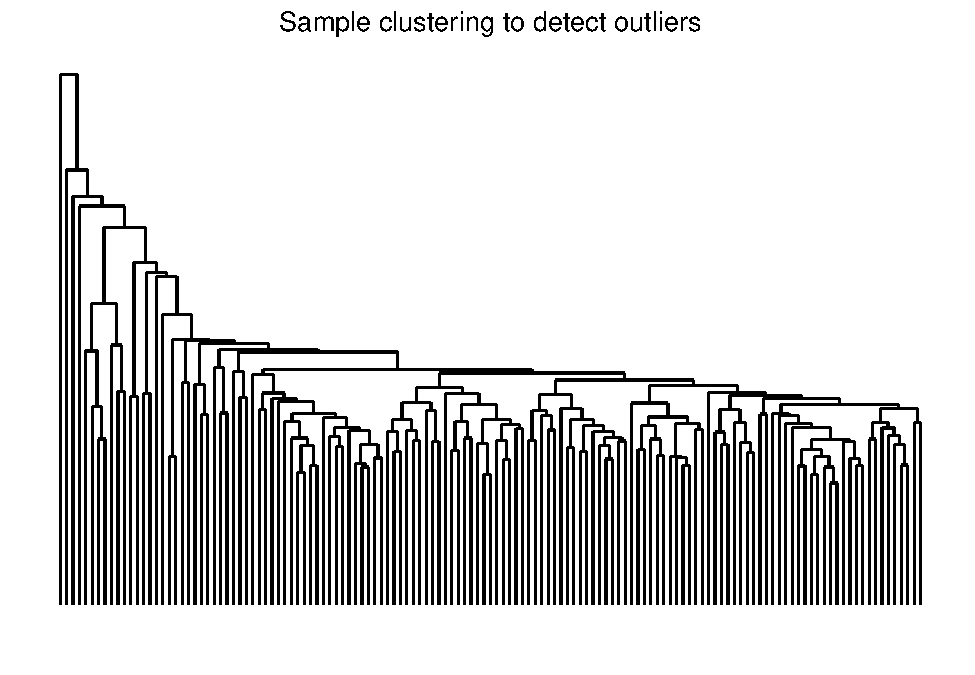
\includegraphics{wgcna_demo_files/figure-latex/clustering samples-1.pdf}


\end{document}
